\documentclass[12pt,a4paper]{article}
\usepackage[utf8]{vietnam}
\usepackage{graphicx}
\usepackage{xcolor}
\usepackage{wrapfig}
\usepackage{multicol}
\usepackage{fancyhdr}
\usepackage{fancybox}
\usepackage{iflang}
\usepackage{caption}
\usepackage{amsmath}
\DeclareMathOperator*{\argmax}{argmax}
\DeclareMathOperator*{\argmin}{argmin}
\usepackage[left=3cm, right=2.50cm, top=2.50cm, bottom=2.50cm]{geometry}
\pagestyle{fancy}
\fancyhf{}
\fancyhead[LE,RO]{\thepage}
\fancyhead[LO]{\small{\itshape{}}}
\graphicspath{ {./images/} }
\begin{document}


	\thispagestyle{empty}
\thisfancypage{
	\setlength{\fboxsep}{10pt}
	\fbox}{}
\begin{center}
	\begin{large}
		TRƯỜNG ĐAI HỌC BÁCH KHOA HÀ NỘI
	\end{large} \\
	\begin{large}
		VIỆN CÔNG NGHỆ THÔNG TIN VÀ TRUYỀN THÔNG
	\end{large} \\
	
	\textbf{--------------------  *  ---------------------}\\[1.5cm]
	
\includegraphics[scale=0.25]{12}
	\\
	\vspace{1.5cm}
	{\fontsize{12pt}{1}\selectfont  Môn học}\\[0.3cm]
	{\fontsize{15pt}{1}\selectfont  Project 2}\\[0.9cm]
	{\fontsize{12pt}{1}\selectfont  Tên đề tài}\\[0.5cm]
	{\fontsize{18pt}{1}\selectfont \textbf{Gợi ý trích dẫn cho các bài báo}}\\[1.3cm]
\end{center}
\vspace{1.5cm}
\hspace{2.7cm}
{\fontsize{12pt}{1}
	\selectfont Giảng viên hướng dẫn: } \hspace{1pt}
\textbf{\parbox[t]{6cm}{
		\selectfont PGS. TS. Nguyễn Kim Anh\\
	}
}

\hspace{2.55cm}
{\fontsize{12pt}{1}
	\selectfont Sinh viên thực hiện: } \hspace{1pt}
\textbf{\parbox[t]{6cm}{
		\selectfont Lâm\ Xuân\ Thư\\
		\selectfont Tống\ Văn\ Vinh\\
	}
}

\hspace{5.0cm}
%{\fontsize{12pt}{1}
%		\selectfont MSSV : } \hspace{1pt}
%	\textbf{\parbox[t]{6cm}{
%			\selectfont  20153709\\
%		}
%	}

\hspace{5.39cm}
{\fontsize{12pt}{1}
	\selectfont Lớp: } \hspace{1pt}
\textbf{\parbox[t]{6cm}{
		\selectfont KSTN\ CNTT\ K60\\
	}
}\\[20pt]

\vspace{1.5cm}
\begin{center}
	
	{\fontsize{12pt}{1}\selectfont Hà Nội, \today}
	%{\fontsize{12pt}{1}\selectfont November, 29$^{th}$, 2017}
\end{center}




\newpage
\thispagestyle{empty}
\tableofcontents 
%\listoffigures
\newpage
\setlength{\parindent}{4em}
\setlength{\parskip}{1em}
\renewcommand{\baselinestretch}{1.5}
\section{Giới thiệu}

Hiện nay với sự phát triển của công nghệ thông tin, có rất nhiều những bài báo điện tử có sẵn trên mạng, số lượng bài báo khổng lồ này trở thành một nguồn dữ liệu giàu có nhưng lại chưa được khai thác hiệu quả và có hệ thống. Bên cạnh những lợi ích có thể đạt được từ việc khai thác nguồn thông tin này, có rất nhiều những thách thức vẫn chưa được giải quyết, (Liu, 2016): 1) Những nhà nghiên cứu cần thu thập thông tin, trích xuất thông tin, và những công cụ gợi ý có thể nhanh chóng lựa chọn ra những bài báo phù hợp với yêu cầu của mình. Những công cụ tìm kiếm các tài liệu khoa học gần đây như Google Scholar và Microsoft Academic bị giới hạn bởi cú pháp truy vấn chuẩn để xác định yêu cầu của người dùng. 2) Việc hiểu nội dung của những bài báo vẫn còn khó khăn. Một người mới tiếp cận tới một vấn đề có thể sẽ cần đọc rất nhiều những tài liệu liên quan tới vấn đề đó, nhưng để thu thập được những tài liệu như thế cần rất nhiều công sức và hiện tại vẫn chưa có công cụ nào đủ mạnh hỗ trợ cho nhu cầu đó. 3) Một vài phát triển thú vị gần đây như CiteRank (Walker, Xie, Yan, $\&$ Maslov, 2007) và Citation Influence Model (Dietz, Bickel, Scheffer, 2007), đã chứng tỏ việc sử dụng thông tin trích dẫn để gợi ý bài báo chất lượng cho người dùng là hoàn toàn khả thi. Tuy nhiên những mô hình đó đều khá đơn giản và chưa khai thác được nhiều thông tin như thông tin về ngữ nghĩa, chủ đề, hoặc sử dụng dữ liệu mạng trích dẫn còn quá đơn sơ khiến hiệu quả gợi ý còn chưa tốt.


Trong Báo cáo Project2 này, nhóm chúng em chủ yếu tập trung vào thực hiện lại những gì mà bài báo (Liu 2016) đã làm. Mặc dù chưa hoàn toàn thực hiện được như những gì bài báo đã làm hay cải tiến được gì thêm, nhưng đây có thể là bước đầu trong quá trình tìm hiểu một vấn đề mới, làm cơ sở cho những phát triển sau này.


Nội dung báo cáo tiếp theo gồm bốn phần chính. Phần một là giới thiệu. Phần hai là cơ sở lý thuyết, bao gồm những kiến thức về các mô hình như Latent Dirichlet Allocation (LDA) và Labelled LDA (LLDA) và thuật toán PageRank. Phần 3 là thực nghiệm, bao gồm mô tả về dữ liệu đã thu thập được và công việc triển khai lập trình, cùng một số kết quả đã đạt được. Phần cuối cùng là kết luận và một số hướng phát triển trong tương lai.


Cuối cùng, chúng em xin gửi lời cảm ơn chân thành tới cô Nguyễn Kim Anh đã rất nhiệt tình dạy bảo, chúng em đã học hỏi được rất nhiều điều mới và thú vị. Chúng em cũng xin gửi lời cảm ơn tới anh Nguyễn Thành Đạt và anh Đinh Xuân Trường đã nhiệt tình giúp đỡ chúng em trong nhiều vấn đề về khai thác dữ liệu cũng như một số thắc mắc về kiến thức khác. Mặc dù những gì đạt được chỉ là dở dang, nhưng vẫn rất hứa hẹn và có nhiều khả năng phát triển. Mong rằng những kết quả này sẽ có ích về sau.


\vspace{1.3cm}
\hspace{9.5cm} Bách Khoa, 03/06/2018


\newpage
\section{Cơ sở lý thuyết}

\subsection{Latent Dirichlet Allocation}
Latent Dirichlet Allocation (LDA), là một mô hình sinh xác suất cho tập dữ liệu rời rạc dựa trên phân phối Dirichlet. LDA là một mô hình Bayesian ba mức, trong đó mỗi phần của mô hình được coi như một mô hình trộn hữu hạn trên cơ sở tập các xác suất của chủ đề. Đối với mô hình hóa văn bản, mỗi xác suất trên các chủ đề có thể đại diện cho một văn bản. Việc mô hình hóa chủ đề thực sự rất có ý nghĩa, nhất là khi muốn vector hóa một văn bản nhưng lại không muốn vector quá thưa hoặc quá nhiều thuộc tính, từ đó có thể dễ dàng thực hiện những thuật toán khác nhau của học máy như phân cụm, phân loại, tóm tắt văn bản,... Để cho thuận tiện, những ký hiệu sau sẽ được sử dụng:


\begin{itemize}
\item Một từ là một đơn vị cơ bản của dữ liệu nằm trong một từ điển, và được đánh chỉ số bởi tập ${1, 2,..., V}$. Mỗi từ sẽ được biểu diễn bởi một "one-hot" vector, trong đó chỉ có một chiều có giá trị bằng một, các chiều còn lại có giá trị bằng 0. Do đó có thể biểu diễn một V-vector từ là $w$ sao cho $w^v = 1$ và $w^u = 0$ với mọi $u$ khác $v$.
\item Một văn bản (document) là một dãy $N$ từ được định nghĩa bởi $\textbf{w} = (w_1, w_2,..., w_N)$, trong đó $w_n$ là từ thứ $n$ trong dãy.
\item Một tập văn bản (corpus) là một tập $M$ văn bản ký hiệu $D = \{\textbf{w}_1, \textbf{w}_2,..., \textbf{w}_M\}$

\end{itemize}
Mục đích là tìm ra một mô hình xác suất cho một corpus không chỉ gán xác suất cho các thành phần của corpus, mà còn gán xác suất cho những document khác.


Ý tưởng cơ bản của LDA là các documents được đại diển bởi việc trộn các chủ đề ẩn, trong đó mỗi chủ đề là một phân phối trên các từ. LDA giả sử quá trình tạo ra một document $\textbf{w}$ trong corpus D diễn ra như sau:

\begin{enumerate}
\item Chọn $N \sim Poisson(\xi)$
\item Chọn $\theta \sim Dir(\alpha)$
\item Với mỗi từ trong N từ của document:

	\begin{enumerate}
	\item Chọn một chủ đề $\textbf{z}_n \sim Multi(\theta)$
	\item Chọn một từ $w_n$ từ $p(w_n | \textbf{z}_n, \beta)$, một phân phối xác suất đa thức có điều kiện là $z_n$
	\end{enumerate}
\end{enumerate}

Một vài giả thiết đã được đưa ra trong mô hình. Đầu tiên, số chiều $k$ của phân phối $Dirichlet$ giả sử đã biết và là một hằng số. Thứ hai, phân phối các từ được tham số hóa bằng một ma trận $\beta$ kích thước $k \times V$, trong đó ${\beta}_j = p(\textbf{w}^j | \textbf{z}^i = 1)$.


Biến ngẫu nhiên $Dirichlet$ $k$ chiều $\theta$ được lấy mẫu từ phân phối $Dirichlet$ với tham số $\alpha$ theo hàm mật độ xác suất sau:

\begin{equation} \label{eq:1}
p(\theta | \alpha) = \dfrac{\Gamma (\sum_{i=1}^{k} {\alpha}_i)}{\prod_{i=1}^{k} \Gamma ({\alpha}_i)} {\theta}_{1}^{{\alpha}_1 - 1}...{\theta}_{k}^{{\alpha}_k - 1}
\end{equation} 


trong đó tham số $\alpha$ là một vector $k$ chiều với các thành phần ${\alpha}_i > 0$, một đặc điểm của phân bố $Dirichlet$ khiến nó hay được sử dụng là nó có tính liên hợp với phân bố đa thức. Phân bố đồng thời của $\theta,$ tập N chủ đề $\textbf{z}$, và tập N từ $\textbf{w}$ được cho bởi công thức:

\begin{equation} \label{eq:2}
p(\theta, \textbf{z}, \textbf{w} | \alpha, \beta) = p(\theta | \alpha) \prod_{n = 1}^{N} p(z_n | \theta)p(w_n | z_n, \beta)
\end{equation} 

\begin{figure}[h]
    \centering
    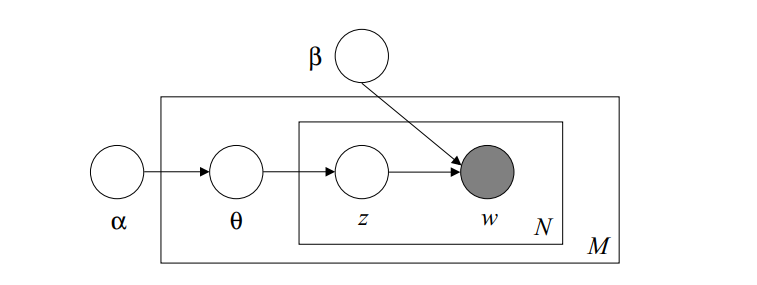
\includegraphics[width=.6\textwidth]{lda}
    \caption{Mô phỏng LDA}
    \label{fig:lda}
\end{figure}
\noindent
trong đó $p(z_n| \theta)$ bằng ${\theta}_i$ để $z_i = 1$. Lấy tích phân trên $\theta$ và lấy tổng trên $z$, ta được phân bố xác suất biên cho một document:

\begin{equation} \label{eq:3}
p(\textbf{w} | \alpha, \beta) = \int p({\theta}| \alpha) \left( \prod_{n=1}^{N} \sum_{z_n} p(z_n | \theta) p(w_n | z_n, \beta) \right)d\theta
\end{equation}

\noindent
Cuối cùng, lấy tích của các xác suất biên của mỗi document ta được hàm mật độ xác suất của corpus:

\begin{equation} 
p(\textbf{D} | \alpha, \beta) = \prod_{d=1}^{M} \int p({\theta}_d | \alpha) \left( \prod_{n=1}^{N_d} \sum_{z_{dn}} p(z_{dn} | {\theta}_d)p(w_{dn} | z_{dn}, \beta) \right) d{\theta}_d
\end{equation}

LDA được mô phỏng bằng hình học như Hình 1, có 3 mức biểu diễn cho mô hình này. Các tham số $\alpha$ và $\beta$ là các tham số mức corpus, giả sử được lấy mẫu một lần trong quá trình tạo corpus. Các biến ${\theta}_d$ là các biến mức document, được lấy mẫu một lần trên mỗi document. Cuối cùng, các biến $z_{dn}$ và $w_{dn}$ là các biến mức từ và được lấy mẫu cho mỗi từ của document.


\subsubsection{LDA và tính khả chuyển}
Một tập biến ngẫu nhiên ${z_1,..., z_N}$ được gọi là khả chuyển nếu phân bố đồng thời của chúng là bất biến với mọi hoán vị. Nếu $\pi$ là một hoán vị của các số tự nhiên từ 1 tới N:

\begin{equation} 
p(z_1, z_2,..., z_N) = p(z_{\pi (1)}, z_{\pi (2)},..., z_{\pi (N)})
\end{equation}


Một dãy vô hạn các biến ngẫu nhiên được gọi là dãy vô hạn khả chuyển nếu mỗi dãy con hữu hạn là khả chuyển. Trong mô hình LDA, ta giả sử các từ được tạo ra bởi các chủ đề và những chủ đề này là dãy vô hạn khả chuyển trong một document. Dựa vào định lý de Finetti, xác suất của một dãy các từ và chủ đề phải có dạng:

\begin{equation} 
p(\textbf{w}, \textbf{z}) = \int p(\theta) \left(\prod_{n=1}^{N} p(z_n | \theta) p(w_n | z_n) \right)d\theta
\end{equation}

\subsubsection{Suy diễn và ước lượng tham số}

Từ những gì đã trình bày, ta có thể thấy ý tưởng đằng sau của LDA, tuy nhiên, những gì chúng ta cần là phải suy diễn và ước lượng được các tham số của mô hình LDA.

\begin{figure}[h]
    \centering
    \captionsetup{justification=centering}
    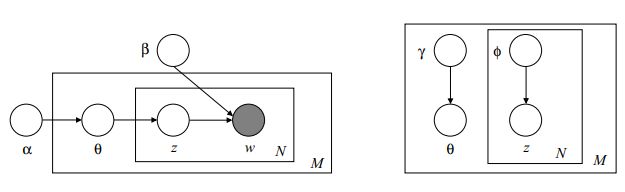
\includegraphics[width=.9\textwidth]{varitional}
    \caption{(Trái) Mô hình đồ thị biểu diễn LDA. (Phải) Mô hình đồ thị biểu diễn suy diễn biến phân được sử dụng để xấp xỉ xác suất hậu nghiệm trong LDA}
    \label{fig:varitional}
\end{figure}

\noindent
Để sử dụng được LDA, chúng ta phải tính được xác suất hậu nghiệm của các biến ẩn đối với một document:

\begin{equation} 
p(\theta, \textbf{z} | \textbf{w}, \alpha, \beta) = \dfrac{p(\theta, \textbf{z}, \textbf{w} | \alpha, \beta)}{p(\textbf{w} | \alpha, \beta)}
\end{equation}

\noindent
Đáng tiếc là phân phối này không tính được. Thực tế, để đơn giản hóa phan phối, ta lấy xác suất biên trên các biến ngãu nhiên và viết lại phương trình (3) với điều kiện là các tham số mô hình:

\begin{equation} 
p(\textbf{w}, | \alpha, \beta) = \dfrac{\Gamma (\sum_i {\alpha}_i)}{\prod_i \Gamma (\alpha_i)} \int \left(\prod_{i=1}^{k} {\theta}_{i}^{{\alpha}_i - 1} \right) \left(\prod_{i=1}^{N} \sum_{i=1}^{k} \prod_{j=1}^{V} (\theta_i {\beta}_{ij})^{w_{n}^{j}} \right)d\theta
\end{equation}

\noindent
một hàm mà không thể tính được bởi cặp $\theta$ và $\beta$ trong công thức tổng trên các chủ đề ẩn (Dickey, 1983).


Mặc dù phân bố hậu nghiệm là không thể tính được cho suy diễn chính xác, có rất nhiều những thuật toán xấp xỉ khác nhau có thể được sử dụng cho LDA, bao gồm xấp xỉ Laplace, suy diễn biến phân, và sử dụng chuỗi Markov (Jordan, 1999). Trong phần này ta sẽ đi sâu vào một thuật toán, đó là suy diễn biến phân lồi.


\subsubsection{Suy diễn biến phân}

Ý tưởng cơ bản của suy diễn biến phân lồi là sử dụng bất đẳng thức Jensen để đạt được một cận dưới khả chỉnh của log likelihood (Jordan et al., 1999). Cụ thể hơn, ta sẽ xét một họ các cận dưới, được đánh chỉ số bởi một tập các tham số biến phân. Các tham số sẽ được chọn sao cho cận dưới đạt được là chặt nhất có thể.


Một cách đơn giản để có được một họ các cận dưới giải được là xét các thay đổi nhỏ của mô hình ban đầu, trong đó một vài cạnh và nút bị xóa. Xét trong trường hợp mô hình LDA được mô tả như Hình 2 (Trái). Sự kết nối mơ hồ giữa $\theta$ và $\beta$ phát sinh bởi các cạnh giữa $\theta$, \textbf{z}, và \textbf{w}. Bằng cách loại bỏ các cạnh đó và nút \textbf{w}, và để lại một mô hình đơn giản với các tham số biến phân tự do, ta có một họ của các phân phối trên các biến ẩn. Họ này được biểu diễn bởi phân phối biến phân sau:


\begin{equation} 
q(\theta , \textbf{z} | \gamma, \phi ) = q(\theta | \gamma) \prod_{n=1}^{N} q(z_n | \phi_n),
\end{equation}

\noindent
trong đó tham số Dirichlet gama và tham số đa thức $(\phi_1, \phi_2, ...\phi_N)$ là các tham số biến phân tự do


Sau khi có được một họ các phân phối xác suất đơn giản, bước tiếp theo là tìm các tham số gama và phi sao cho cận dưới của log likelihood là nhỏ nhất. Điều đó dẫn đến nhu cầu giả bài toán tối ưu sau:


\begin{equation} 
(\gamma^{*}, \phi^{*}) = \argmin_{(\gamma, \theta)} D(q(\theta, \textbf{z} | \gamma, \phi) || p(\theta, \textbf{z} | \textbf{w}, \alpha, \beta))
\end{equation}

\noindent
Do đó giá trị tối ưu của các tham số biến phân được tìm bởi việc tối thiểu hóa Kullback-Leibler giữa phân phối biến phân và xác suất hậu nghiệm thực tế $p(\theta, \textbf{z}| \textbf{w}, \alpha, \beta)$. Sự tối thiểu hóa này có thể đạt được thông qua phương pháp điểm cố định lặp. Cụ thể, bằng cách tính đạo hàm của KL và cho giá trị đạo hàm này bằng 0, ta được cặp phương trình cập nhật sau:


\begin{equation} 
\phi_{ni} \propto \beta_{iw_n} exp \{ E_q [ log(\theta_i)| \gamma ] \} 
\end{equation}
\begin{equation} 
\gamma_i = \alpha_i + \sum_{n=1}^{N} \phi_{ni}
\end{equation}


\noindent
Giá trị kỳ vọng trong cập nhật đa tức có thể được tính như sau:

\begin{equation} 
E_q [ log(\theta_i) | \gamma ] = \Psi (\gamma_i) - \Psi \left(\sum_{j=1}^{k} \gamma_j \right)
\end{equation}

\noindent
Trong đó $\Psi$ là đạo hàm cấp một của hàm log($\Gamma$), có thể tính được bằng xấp xỉ Taylor (Abramowitz và Stegun, 1970)


Chú ý rằng phân phối biến phân thực ra là xác suất có điều kiện, thay đổi bởi hàm của \textbf{w}. Điều này xảy ra bởi bài toán tối ưu (10) đã giả sử \textbf{w} là cố định, do đó có được các tham số tối ưu $(\gamma^{*}, \phi^{*})$ là hàm của \textbf{w}. Chúng ta có thể viết kết quả của phân phối biến phân là $q(\theta, \textbf{z} | \gamma^{*} (\textbf{w}), \phi^{*} (\textbf{w}))$. Do đó phân bố biến phân có thể được xem như một xấp xỉ cho phan bố hậu nghiệm $p(\theta, z| w, \alpha, \beta)$. Ta tổng hợp suy diễn biến phân như hình (3).

\begin{figure}[h]
    \centering
    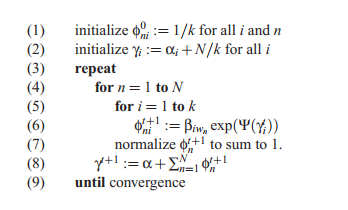
\includegraphics[width=.6\textwidth]{vi}
    \caption{Một giải thuật suy diễn biến phân cho LDA}
    \label{fig:vi}
\end{figure}

\subsubsection{Ước lượng tham số}
Phần này sẽ trình bày một phương pháp Bayes để ước lượng tham số cho mô hình LDA. Trong trường hợp cụ thể, với corpus $D = {w_1, w_2, ..., w_M}$, chúng ta muốn tìm các tham số $\alpha$ và $\beta$ để cực đại hóa log likelihood của dữ liệu:

\begin{equation} 
l (\alpha, \beta) = \sum_{d=1}^{M} log p (\textbf{w}_d | \alpha, \beta)
\end{equation}

\noindent
Như đã mô tả bên trên, giá trị $p(\textbf{w}, \alpha, \beta)$ không thể tính toán chính xác được. Tuy nhiên, suy diễn biến phân cung cấp cho chúng ta một cận dưới có thể tính được của hàm log likelihood, một cận dưới mà có thể tối ưu trên $\alpha$ và $\beta$. Từ đó có thẻ tìm một ước lượng Bayes xấp xỉ cho mô hình LDA, tìm ra được cận dưới phù hợp nhất bằng cách chỉ ra giá trị phù hợp của gama và phi, sau đó với các tham số biến phân đã tìm được, ta tối đa hóa cận dưới này đối với các tham số $\alpha$ và $\beta$.


Như vậy, về mặt chi tiết, với việc sử dụng thuật toán Expectation Maximization (EM), ta sẽ tìm được các tham số phù hợp với yêu cầu của bài toán:

\begin{enumerate}
\item (E-step) Với mỗi document, tìm giá trị tối ưu của các tham số biến phân $\{ \gamma_d^{*}, \phi_d^{*} : d \in D\}$. Cách làm đã được đưa ra ở phần trước.

\item (M-step) Tối ưu hóa cận dưới tìm được đối với các tham số $\alpha$ và $\beta$. Việc này tương đương với tìm MLE với kỳ vọng thống kê đủ cho mỗi document với xấp xỉ hậu nghiệm được tính ở E-step.

\end{enumerate}

\begin{figure}[h]
    \centering
    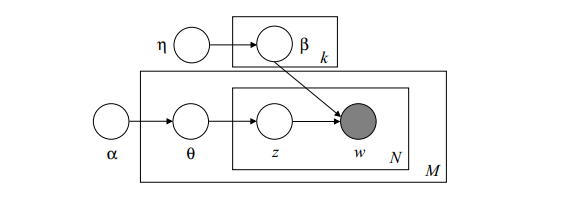
\includegraphics[width=.8\textwidth]{smoothlda}
    \caption{Mô hình LDA trơn}
    \label{fig:smoothlda}
\end{figure}

\noindent
Hai bước trên được lặp cho đến khi cận dưới của log likelihood hội tụ.

\subsubsection{Làm trơn mô hình LDA}

Kích thước của từ điển thường rất lớn, dẫn đến nhiều vấn đề gây ra bởi sự thưa của các vector và ma trận. Một document mới rất có thể sẽ chứa những từ mà chưa xuất hiện trong bất kỳ document nào trước đó. Ước lượng MLE của các tham số đa thức gán xác suất bằng 0 cho những từ như thế, và vì vậy, gán xác suất bằng 0 cho document mới. Một cách tiếp cận hợp lý là "làm trơn" các tham số đa thức, gán giá trị xác suất dương cho tất cả các từ trong từ điển cho dù nó có được quan sát ở tập luyện hay không (Jelinek, 1997). phương pháp làm trơn Laplace thường được sử dụng; Điều này về cơ bản mang lại giá trị tủng bình của phân phối hậu nghiệm dưới một tiên nghiệm Dirichlet đều trên các tham số đa thức.


Không may, trong mô hình trơn, phương pháp làm trơn Laplace không còn là một phương pháp hợp lý. Thực tế, bằng việc đặt một tiên nghiệm Dirichlet cho các tham số đa thức, ta được một hậu nghiệm không tính được, cũng như hậu nghiệm không tính được của mô hình LDA đơn giản. Giải pháp đề xuất cho vấn đề này là áp dụng suy diễn biến phân cho mô hình mở rộng đã bao gồm làm trơn Dirichlet trên tham số đa thức.


Với mô hình LDA, ta được mô hình mở rộng như trong hình (4), một trong những lợi ích của LDA so với những mô hình biến ẩn liên quan là nó cung cấp một suy diễn rõ ràng cho những documents chưa được quan sát.


\subsubsection{Mô hình LDA có nhãn}

Thực tế có rất nhiều văn bản đã được gán nhãn bởi người đọc hoặc tác giả. Đối với các bài báo thì nhãn có thể là các từ khóa đi kèm với bài báo. Mô hình LDA đơn giản chưa khai thác được đặc điểm này của các document. Từ đó mô hình LDA có nhãn ra đời.


Mô hình LDA thông thường được xem như một thuật toán học phi giám sát. Nó đơn thuần làm việc trên dữ liệu không có nhãn nên kết quả đem lại thường không có độ chính xác cao. Mô hình LDA có nhãn (Deniel Ramage, 2009) ngược lại, là một thuật toán học có giám sát, sử dụng các nhãn có sẵn của mỗi document để cải thiện khả năng học chủ đề của mình.

\begin{figure}[h]
    \centering
    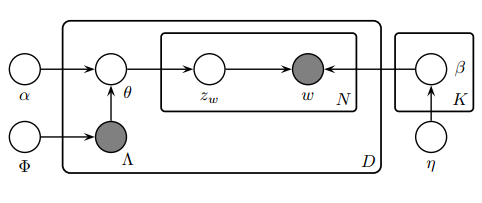
\includegraphics[width=.8\textwidth]{llda}
    \caption{Mô hình LDA có nhãn}
    \label{fig:llda}
\end{figure}


Mô hình LDA có nhãn được mô tả một cách trực quan bằng đồ thị trên hình 5. Có thể thấy, giống như LDA, LLDA mô hình hõa mỗi document bằng một tổ hợp các chủ đề và tạo ra từng từ một từ mỗi chủ đề đó. Nhưng cái khác của LLDA là nó kết hợp thông tin có giám sát bằng cách ràng buộc mô hình chủ đề chỉ sử dụng những chủ đề tương ứng với một tập các nhãn của một document.

\newpage
Ta đặt số lượng chủ đề trong LLDA bằng số lượng chủ đề K trong corpus. Quá trình sinh cho thuật toán được mô tả bằng mã giả như sau:

\begin{figure}[h]
    \centering
    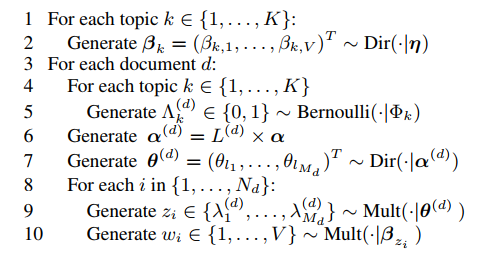
\includegraphics[width=.6\textwidth]{lldapseudo}
    \caption{Mã giả cho mô hình sinh LLDA}
    \label{fig:lldapseudo}
\end{figure}

Ở đây, quá trình suy diễn để tìm các tham số cho mô hình LLDA khá phức tạp nên sẽ không trình bày cụ thể.

\newpage
\subsection{Giải thuật PageRank}
\subsubsection{Giải thuật PageRank gốc}
PageRank là thuật toán phân tích các liên kết được dùng trong Google Search để xếp hạng các trang web. Ý tưởng chính của PageRank khá đơn giản, một trang web được coi là quan trọng nếu nó được trích dẫn bởi những trang quan trọng khác. Ví dụ, nếu một trang web j có rất nhiều trang web khác link tới nó, thì có thể coi trang web j là một trang quan trọng.


\begin{figure}[h]
    \centering
    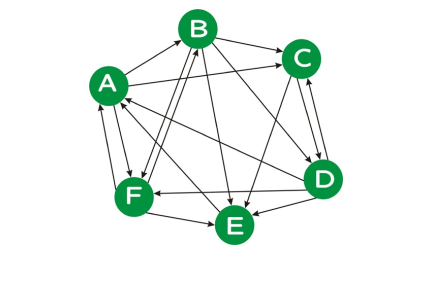
\includegraphics[width=.4\textwidth]{pagerank}
    \caption{Mã giả cho mô hình sinh LLDA}
    \label{fig:lldapseudo}
\end{figure}

Giả sử trong trường hợp cụ thể, chúng ta có một đồ thị có hướng chỉ có 6 nút. Khi nút $i$ trích dẫn nút $j$, ta thêm một cạnh có hướng giữa $i$ và $j$ trên đồ thị. Trong mô hình PageRank, mỗi nút sẽ truyền độ quan trọng của nó cho những nút mà nó link đến. Ví dụ, trang A có 3 cạnh hướng ngoại, do đó nó sẽ truyền $1/3$ độ quan trọng cho các nút B, C, và F. Thông thường, nếu một nút có $k$ cạnh hướng ngoại, nó sẽ truyền $1/k$ độ quan trọng của nó cho mỗi trang mà nó link đến. Theo như luật truyền này, chúng ta có thể định nghĩa ma trận chuyển tiếp của đồ thị P:

$$
P = 
\begin{bmatrix}
    0 & 0 & 0 & \frac{1}{4} & 1 & \frac{1}{3} \\
    \frac{1}{3} & 0 & 0 & 0 & 0 & \frac{1}{3} \\
    \frac{1}{3} & \frac{1}{4} & 0 & \frac{1}{4} & 0 & 0 \\
    0 & \frac{1}{4} & \frac{1}{2} & 0 & 0 & 0 \\
    0 & \frac{a}{4} & \frac{1}{2} & \frac{1}{4} & 0 & \frac{1}{3} \\
    \frac{1}{3} & \frac{1}{4} & 0 & \frac{1}{4} & 0 & 0
\end{bmatrix}
$$

Bắt đầu với phân phối đều, tầm quan trọng của mỗi node là 1/6. Gọi $\pi$ là giá trị PageRank khởi tạo, có tất cả các chiều bằng 1/6. Bởi mỗi link tới tăng giá trị PageRank của một nút, chúng ta cập nhật xếp hạng của mỗi nút bằng việc cộng giá trị hiện tại với độ quan trọng của các link tới. Công thức cập nhật giá trị pagerank như sau:

$$
r^{t+1}(i) = \sum_{j \in E(i)} \dfrac{r^t (j)}{I(j)}
$$

\noindent
trong đó $r^{t}(i)$ là giá trị pagerank của nút $i$ tại thời điểm $t$ còn $I(j)$ là số link hướng ngoại của nút $j$. Từ đó các giá trị pagerank của từng nút sẽ được cập nhật qua từng vòng lặp. Ở vòng lặp đầu tiên, ta chỉ đơn giản là nhân ma trận P với ma trận $\pi$, ở các lần cập nhật tiếp theo, ta cũng chỉ cần nhân ma trận P với các giá trị đã cập nhật trước đó. Khi số vòng lặp đủ lớn, ta có kết quả là pagerank của cả đồ thị đã cho.

$$
\pi = 
\begin{bmatrix}
    0.167 \\
    0.167 \\
    0.167 \\
    0.167 \\
    0.167 \\
    0.167 
\end{bmatrix} , 
P\pi = 
\begin{bmatrix}
	0.264 \\
	0.111 \\
	0.139 \\
	0.125 \\
	0.222 \\
	0.139
\end{bmatrix} ,
P^2\pi =
\begin{bmatrix}
	0.300 \\
	0.134 \\
	0.147 \\
	0.097 \\
	0.175 \\
	0.147
\end{bmatrix} ,..., 
P^{13} = 
\begin{bmatrix}
	0.265 \\
	0.138 \\
	0.150 \\
	0.111 \\
	0.187 \\
	0.150
\end{bmatrix}
$$

\noindent
Như vậy, ta cứ tiếp tục thực hiện vòng lặp cho đến khi đạt được giá trị hội tụ theo ngưỡng mong muốn. Giá trị này cũng là gía trị PageRank vector của cả mạng đã cho.


\subsubsection{PageRank cải tiến với tri thức tiên nghiệm}
Trong bài toán $ Citation $, chúng ta sử dụng thuật toán PageRank cải tiến để tính toán tiên nghiệm publication topic (publication topic prior). Với mỗi topic khác nhau, (tiên nghiệm) độ quan trọng có thể khác nhau.

Với mỗi topic cho trước $ z_{key_{t}} $, xác suất tiên nghiệm đỉnh $ p_{z_{key_{t}}} $ đối với nhiều publication có thể bằng không. Vì vậy, với mỗi topic, thuật toán PageRank cải tiến có thể đưa ra độ "độ quan trọng liên quan" của các đỉnh trong đồ thị G xét với tập các đỉnh gốc $  R \subseteq V $, trong đó với mỗi $ r  $ nằm trong R thì $ p_{r, z_{key_{t}}} \neq 0 $. Các đỉnh gốc này có thể xem như các publication quan trọng đối với một topic cho trước (\textit{tri thức tiên nghiệm}). 

Công thức PageRank cải tiến sử dụng tri thức tiên nghiệm tính giá trị độ quan trọng liên quan của các đỉnh, $ I_{key_{t}}(v|R) = \pi_{key_{t}}(v) $, và:

\begin{figure}[h]
	\begin{center}
		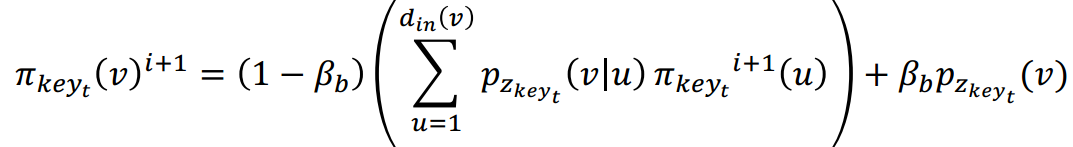
\includegraphics[scale=0.4]{cong_thuc_pr} 
		%\caption{Ví dụ tính PageRank 2}
	\end{center}
\end{figure}

Công thức này mô tả một chuỗi Markov cho một "surfer" ngẫu nhiễn với xác suất chuyển về tập gốc R là $ \beta_{b} $ tại mỗi bước. Việc thêm phần cuối của công thức trên so với công thức của PageRank nguyên bản đồng thời giúp vượt qua được trường hợp $ rank sink $. $ p_{z_{key_{t}}(v|u)} $ là xác suất chuyển từ u sang v.

Kết quả thu được có dạng như hình 8.

\begin{figure}[h]
	\begin{center}
		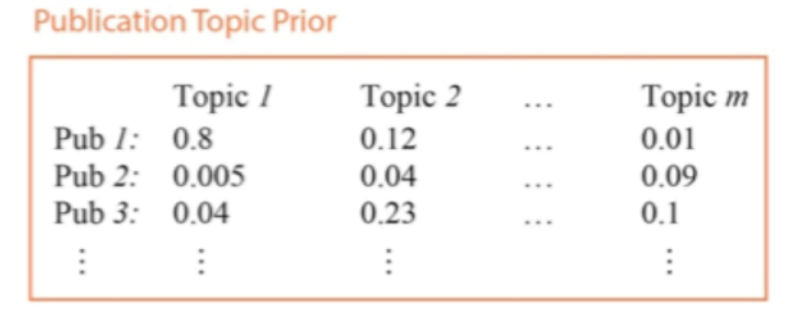
\includegraphics[scale=0.4]{ket_qua_pr} 
		\caption{Publication Topic Prior}
	\end{center}
\end{figure}

\newpage

\subsection{Quay trở lại bài toán trích dẫn}
Phát biểu bài toán: "Giả sử một người muốn tìm các bài báo có liên quan tới vấn đề mà họ đang viết để tham khảo và làm tài liệu trích dẫn, làm sao có thể thiết kế một hệ gợi ý đủ tốt để dựa vào những gì mà người dùng đã viết (tiêu đề, abstract,...), gợi ý cho họ tài liệu phù hợp".


Như vậy, đầu vào của bài toán chỉ là một bản nháp và các thông tin liên quan tới bài báo còn dở dang, mục đích của hệ thống cần xây dựng là trả về những bài báo có liên quan nhất. Có khá nhiều những công trình nghiên cứu khác nhau đã được đưa ra để giải quyết bài toán này, xong những thông tin mà các công trình này khai thác lại khác nhau. Từ những phương pháp cổ điển như tập trung khai thác dữ liệu dạng text (sử dụng TF-IDF hoặc LDA) rồi sử dụng độ tương đồng cosine để giải quyết bài toán gợi ý cho đến những công trình khai thác nhiều thông tin hơn như thông tin về mạng trích dẫn, thông tin về text, kết hợp cả thông tin về ngữ cảnh trích dẫn (Liu et al 2016) rồi sử dụng suy diễn Bayes để gợi ý bài báo phù hợp.  Trong khi chúng ta có rất nhiều thông tin, câu hỏi đặt ra là liệu chúng ta có thể khai thác được hết tất cả những thông tin giàu có mà ta có để cải thiện khả năng giải quyết bài toán ban đầu.


Thông tin để khai thác còn nhiều, công cụ có thể sử dụng thì rất đa dạng, nhưng trong phạm vi một kỳ học, vẫn chưa có ý tưởng mới nào được đưa ra hay cài đặt. Phạm vi của kết quả đã đạt được chỉ là những bước đi thô sơ đầu tiên để hiểu hơn về cách làm của những công trình trước đó, làm bước đệm cho các phát triển sau này. Phần tiếp theo sẽ trình bày về những gì mà nhóm chúng em đã làm trong thời gian nghiên cứu.

\newpage
\section{Thực nghiệm}
\subsection{Dữ liệu}
Trong quá trình tìm kiếm dữ liệu, có hai bộ dữ liệu mà nhóm em có cơ hội được sử dụng. Một là bộ dữ liệu CiteSeer, và bộ dữ liệu thứ hai là OpenCorpus.

\subsubsection{CiteSeerX}
Về bộ dữ liệu CiteSeerX, đó là bộ dữ liệu gồm một lượng lớn các bài báo (630202 bài báo) được lưu dưới dạng text. thông tin cung cấp gồm có full text của mỗi bài báo, đính kèm theo mỗi bài báo còn có tương ứng một file meta data của bài báo đó. 

Trong file metadata có các thông tin về bài báo như Tiêu đề, Tên các tác giả, Abstract, các trích dẫn đi kèm tên của các bài báo được trích dẫn và ngữ cảnh trích dẫn, thông tin về hội nghị, năm xuất bản. 


\begin{figure}[h]
    \centering
    \captionsetup{justification=centering}
    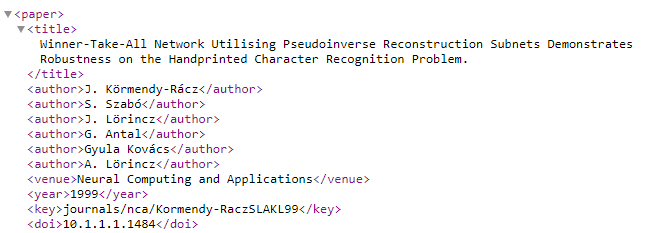
\includegraphics[width=1.\textwidth]{title_paper}
    \caption{Thông tin về tiêu đề, tác giả, năm xuất bản, hội nghị, tạp chí,...}
    \label{fig:title_paper}
\end{figure}

\noindent
Hình 9 là một số thông tin được cung cấp bởi file meta data tương ứng với một file full text của một bài báo. Nhìn chung các thông tin được đưa ra một cách khá rõ ràng, tuy nhiên thông tin về tác giả lại chỉ có tên của tác giả mà không có id tương ứng, chính vì thế việc khai thác thông tin về tác giả, nếu muốn, sẽ rất khó khăn. Thứ hai, đó là thông tin trong trường <key>, thông tin này còn khá là mơ hồ, không có nhiều giá trị khai thác. Các thông tin khác có thể khai thác được là tiêu đề, năm xuất bản, và thông tin trong trường <doi> có thể được dùng làm id của bài báo.

\begin{figure}[h]
    \centering
    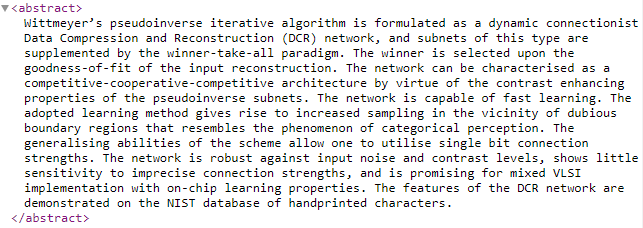
\includegraphics[width=1.\textwidth]{abstract}
    \caption{Nội dung text của abstract của bài báo}
    \label{fig:title_paper}
\end{figure}

\newpage
\noindent
Hình 10 là thông tin về abstract của bài báo, thông tin này khá rõ ràng, và có thể khai thác được.



\begin{figure}[h]
    \centering
    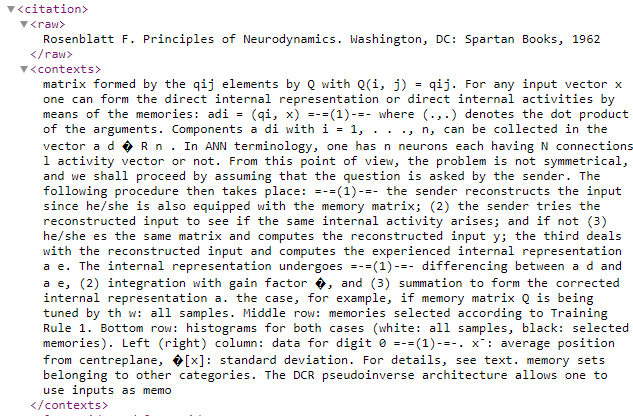
\includegraphics[width=1.\textwidth]{citation}
    \caption{Nội dung của một trích dẫn của bài báo}
    \label{fig:title_paper}
\end{figure}


Hình 11 thể là toàn bộ thông tin của một trích dẫn của bài báo. Thông tin này bao gồm trường <raw> là tên của bài báo cùng với tên tác giả , năm phát hành,... Tuy nhiên điều mấu chốt là id của bài báo mà nó trích dẫn lại không được đưa vào. Từ đó nếu muốn khai thác thông tin dạng mạng thì sẽ phải làm bằng tay, điều này cũng là một thách thức vì thông tin trong trường <raw> thì thực sự là rất thô, có thể thông tin này trong các bài báo khác cũng không được rõ ràng, sử dụng để tìm kiếm id của bài báo tương ứng có thể đem lại kết quả không tốt. Về thông tin về ngữ cảnh trích dẫn thì dài ngắn khác nhau đối với từng bài báo, không có một chuẩn mực nào về số lượng từ được lấy xung quanh vị trí trích dẫn. Nội dung ngữ cảnh cũng khá là nhiễu bởi chứa nhiều kí tự lạ.


\noindent
Vì số lượng các bài báo trong dữ liệu quá lớn nên chúng em chỉ trích xuất một lượng nhỏ các bài báo ra để khảo sát về dữ liệu. Tổng số bài báo được khảo sát là 11396 (khoảng 2\% dữ liệu gốc) để phục vụ nghiên cứu.


Trong quá trình khảo sát đữ liệu, chúng em phát hiện ra dữ liệu còn rất thô và chưa được tiền xử lý tốt, có rất nhiều những bài báo nội dung bị lỗi, và việc lọc bỏ những bài báo lỗi này mới chỉ dừng ở mức loại những bài báo quá ngắn. 


\begin{figure}[h]
    \centering
    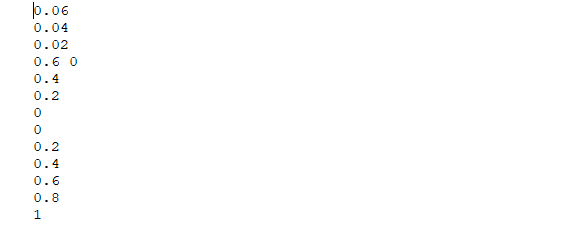
\includegraphics[width=1.\textwidth]{wrong}
    \caption{Một bài báo có nội dung fulltext bị lỗi}
    \label{fig:wrong_paper}
\end{figure}


\subsubsection{Open Corpus}
Về bộ dữ liệu Open Corpus, đây là một bộ dữ liệu khổng lồ gồm 39 triệu bài báo liên quan đến lĩnh vực khoa học máy tính, khoa học thần kinh và y học. Mỗi bài báo được xử lý và trích xuất ra khá nhiều thông tin, mặc dù không có dữ liệu fulltext, nhưng dữ liệu đã được tiền xử lý khá tốt và có tính tin cậy cao, dễ khai thác.

\begin{figure}[h]
    \centering
    \captionsetup{justification=centering}
    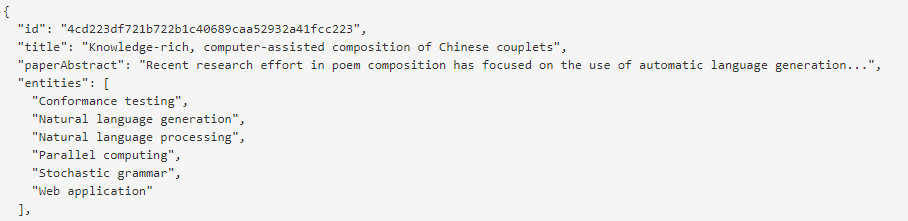
\includegraphics[width=1.\textwidth]{opencorpus1}
    \caption{ID, tiêu đề, abstract, cùng một số nhãn liên quan tới nội dung của bài báo}
    \label{fig:opencorpus1}
\end{figure}

\noindent
Hình 13 mô tả một phần của dữ liệu, thông tin gồm có id của bài báo, tiêu đề, abstract, cùng với một số nhãn được gán cho bài báo nằm trong trường "entities", có thể thấy những thông tin này khá rõ ràng và dễ khai thác.


\begin{figure}[h]
    \centering
    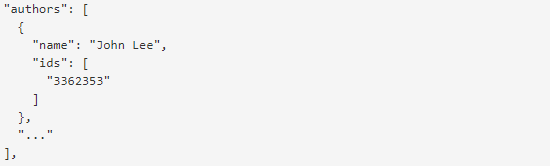
\includegraphics[width=1.\textwidth]{author}
    \caption{Trường tác giả của bài báo}
    \label{fig:author}
\end{figure}

\noindent
Hình 14 mô tả trường tác giả của bài báo, trường này cũng khá chi tiết, và đặc biệt là thông tin về tác giả được gán ID, như vậy ta có thể khai thác thông tin về đồng tác giả đối với dữ liệu này.

\begin{figure}[h]
    \centering
    \captionsetup{justification=centering}
    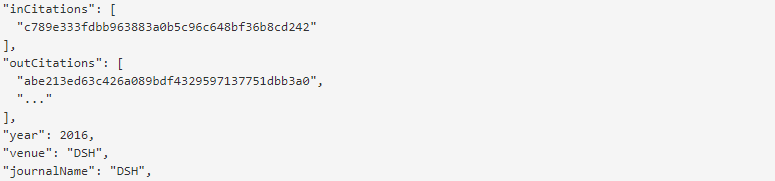
\includegraphics[width=1.\textwidth]{opencorpus2}
    \caption{Một số thông tin khác}
    \label{fig:opencorpus2}
\end{figure}


\noindent
Cuối cùng, hình 15 mô tả những thông tin về các id của những bài báo mà bài báo này trích dẫn, cũng như cả những id của những bài báo trích dẫn bài báo này. Như vậy việc khai thác thông tin mạng trích dẫn cũng hoàn toàn có thể dễ dàng thực hiện được. Ngoài ra, còn có các thông tin về năm xuất bản, tên tạp chí, hội nghị. Những thông tin này cũng rất rõ ràng và dễ khai thác.


Cũng như đối với CiteSeerX, chúng em trích một phần dữ liệu của OpenCorpus ra để làm thực nghiệm, bao gồm tổng cộng 57513 bài báo (gấp hơn 5 lần dữ liệu thực nghiệm của CiteSeerX)

\subsection{Một số cài đặt trên dữ liệu}
\subsubsection{Tiền xử lý dữ liệu}

Tiền xử lý dữ liệu là công đoạn đầu tiên, cũng là công đoạn quan trọng nhất, quyết định thành công của những mô hình áp dụng lên nó sau đó. Tuy nhiên, công đoạn này cũng rất khó khăn, nhất là khi dữ liệu gốc quá thô và nhiễu. 


Đặc thù của dữ liệu cho bài toán này là dữ liệu thuần dạng văn bản. Sản phẩm cuối cùng là dữ liệu đã xử lý gồm có một bộ từ điển, đi kèm là một tập corpus tương đối "sạch". Các công đoạn tiền xử lý dữ liệu diễn ra như sau:

\begin{enumerate}
\item Với mỗi document, chuyển dữ liệu từ dạng string sang một danh sách các từ được sắp thứ tự đúng như thứ tự xuất hiện các từ trong  gốc.
\item Sau khi tách từ, bước tiếp theo là loại bỏ những stopwords khỏi danh sách các từ
\item Tiếp theo là loại bỏ những từ xuất hiện đúng một lần trong document, loại bỏ những từ xuất hiện trong ít hơn 5 document và nhiều hơn 40\% các document (đối với CiteSeer); loại bỏ những từ xuất hiện trong ít hơn 100 document và nhiều hơn 80\% các document (với dữ liệu OpenCorpus)
\item Trong corpus, nếu cặp từ nào xuất hiện cùng nhau trên 20 lần thì cặp từ đó sẽ được kết nối với nhau bằng ký tự \_ tạo thành một từ duy nhất. Ví dụ: từ machine thường đi với từ learning, thì sẽ được ghép thành cụm machine{\_}learning.
\end{enumerate}

\noindent
Sau đây là một số thống kê với dữ liệu trước và sau tiền xử lý:

\begin{figure}[h]
    \centering
    \captionsetup{justification=centering}
    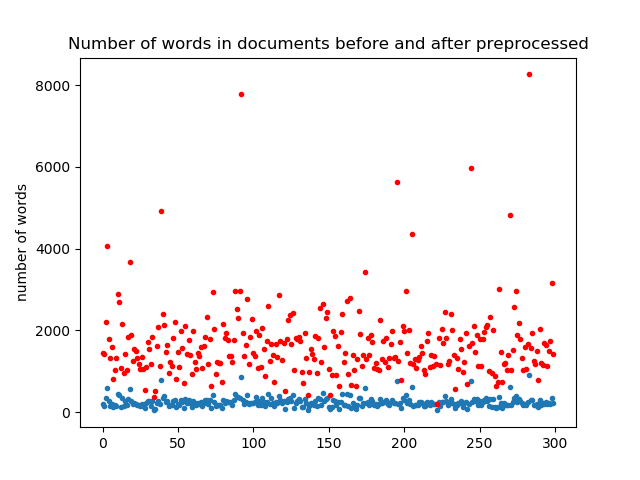
\includegraphics[width=0.9\textwidth]{num_words}
    \caption{Thống kê số từ duy nhất trước và sau tiền xử lý với 300 bài báo fulltext được lấy từ dữ liệu CiteSeer}
    \label{fig:num_words}
\end{figure}
	
\noindent
Hình 16 là thống kê về số từ duy nhất trong mỗi bài báo trước và sau khi tiền xử lý. Trục tung chỉ số lượng từ duy nhất, trục hoành chỉ số thứ tự của bài báo. Mỗi bài báo sẽ được đại diện bởi một điểm xanh và một điểm đỏ, trong đó điểm xanh là số lượng từ duy nhất của bài báo sau tiền xử lý, và điểm đỏ là số lượng từ duy nhất của bài báo trước khi tiền xử lý. Có thể thấy, nhìn chung thì mỗi bài báo trước khi tiền xử lý có số lượng từ duy nhất khá lớn, nhựng chủ yếu taampj trung quanh khoảng 1500 từ tới 2000 từ. Nhưng sau khi tiền xử lý thì chỉ còn khoảng 200 tới 300 từ. Khi lấy các giá trị trung bình thì ta được hình sau:

\begin{figure}[h]
    \centering
    \captionsetup{justification=centering}
    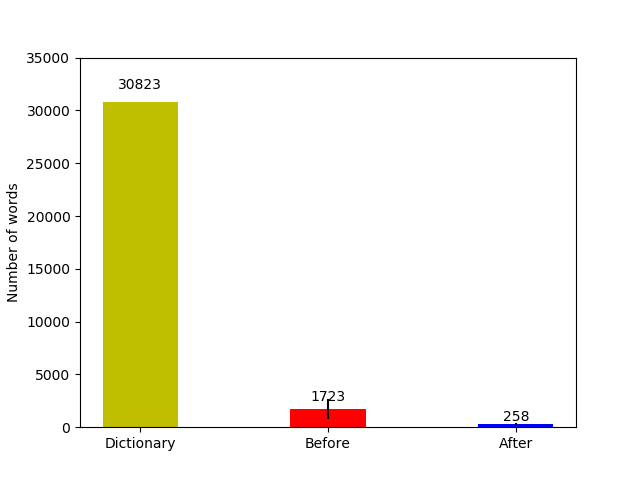
\includegraphics[width=0.9\textwidth]{means}
    \caption{Các giá trị về số từ trong từ điển, cùng với giá trị trung bình thống kê của số từ duy nhất}
    \label{fig:means}
\end{figure}

Có thể thấy, số lượng từ trong từ điển đối với dữ liệu CiteSeerX là 30823 từ, gấp 17 lần số từ duy nhất trước tiền xử lý của mỗi bài báo, và gấp 119 lần số từ duy nhất sau tiền xử lý của mỗi bài báo. Như vậy, nếu biểu diễn mỗi từ bằng một "one-hot" vector thì vector đó là cực kỳ thưa. Và mỗi bài báo nếu được biểu diễn cũng bằng vector có số chiều bằng số chiều trong từ điển thì vector tương ứng cũng vẫn còn quá thưa, với mật độ 0.87%.


Với dữ liệu OpenCorpus, vì chúng ta chỉ làm việc với fulltext là abtract của bài báo nên những tham số thống kê sẽ có đặc điểm khác với dữ liệu CiteSeerX. Đối với dữ liệu OpenCorpus, số lượng bài báo được xem xét là 57513 bài, số lượng từ trong từ điển là 48422 từ, trung bình mỗi abstract, sau tiền xử lý, còn lại khoảng 78 từ duy nhất.


\subsection{Vector hóa dữ liệu}
Do thời gian có hạn nên nhóm mới chỉ khai thác dữ liệu text ở hai bộ dữ liệu. Đó là fulltext ở CiteSeer và abstract ở OpenCorpus. Cũng chính vì mới làm việc với dữ liệu text, cho nên những phương pháp vector hóa cũng chỉ liên quan tới vector hóa dữ liệu text mà thôi.


Có khá nhiều hướng có thể khai thác để vector hóa một văn bản nói chung và dữ liệu text của một bài báo nói riêng. Hướng đơn giản nhất có thể nghĩ đến đó là sử dụng vector với số feature bằng số từ trong từ điển. Với mỗi từ xuất hiện trong document, vị trí tương ứng của nó trong vector sẽ khác không, và có trọng số tỉ lệ với số lần xuất hiện từ đó trong document. Cách làm này thực thế rất kém hiệu quả, vì vector đạt được thường rất thưa và nghèo nàn về mặt ngữ nghĩa. Cách làm thứ hai có thể nghĩ đến là sử dụng TF-IDF để vector hóa văn bản, cách làm này có thể nhanh chóng chọn ra một tập các từ có độ quan trọng cao, đại diện cho một văn bản. Vector hóa sử dụng TF-IDF thường được sử dụng cho những bài toán học có giám sát, người lại với những bài toán học không giám sát, một phương pháp khác tỏ ra khá hiệu quả, đó là sử dụng LDA để mô hình hóa chủ đề cho mỗi văn bản. Với việc mô hình hóa chủ đề, mỗi document sẽ tương ứng với một phân bố xác suất trên các chủ đề, mà số lượng chủ đề thường rất nhỏ khoảng vài chục cho tới vài trăm chủ đề (rất nhỏ so với số lượng các từ trong từ điển) và mỗi thành phần của vector lúc này rất giàu ý nghĩa. 



Với bộ dữ liệu CiteSeer, nhóm cũng đã cố gắng cài đặt mô hình LDA, sử dụng mô hình LDA với 50 chủ đề được suy diễn. Tuy nhiên kết quả suy diễn không được quá khả quan và rõ ràng. Sau đây là 5 topic, mỗi topic gồm 6 từ có xác suất lớn nhất thuộc vào tocpic đó

\begin{figure}[h]
    \centering
    \captionsetup{justification=centering}
    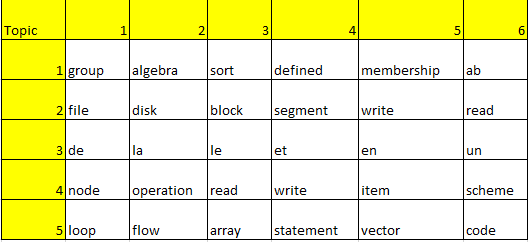
\includegraphics[width=0.9\textwidth]{topicsLDA}
    \caption{5 trong số 50 topics được suy diễn bằng LDA từ dữ liệu CiteSeerX}
    \label{fig:topicsLDA}
\end{figure}

\noindent
Có thể thấy các từ trong mỗi chủ đề chưa thực sự liên quan với nhau và cùng nói về một vấn đề thực tế nào đó. Như vậy, LDA tỏ ra chưa tốt với việc suy diễn chủ đề từ tập dữ liệu này. Do đó, nhóm cũng cố gắng khai thác mô hình khác để giải quyết bài toán này, đó là mô hình LLDA. Tuy nhiên, với mô hình LLDA, cần phải có một tập các nhãn cho mỗi bài báo, nhưng xem xét trong dữ liệu, chỉ có thông tin về các tạp chí là có thể phần nào khai thác được. Nhưng thông tin về các tạp chí ở dữ liệu hầu hết là viết tắt, nên bước đầu tiên là phải dịch hết toàn bộ nội dung viết tắt ra. Rồi sử dụng thuật toán phân cụm để phân cụm các tạp chí, hội nghị có liên quan lại với nhau. Đầu tiên nhóm lựa chọn thuật toán K-means để giải quyết vấn đề phân cụm. Nhưng với LDA có nhãn, mỗi document thường là có nhiều hơn một nhãn, nên nếu sử dụng K-means, thì mỗi bài báo chỉ có một nhãn duy nhất. Do vậy, cần phải tìm một phương pháp phân cụm khác, mềm dẻo hơn. Một trong những phương pháp có thể xem xét trong tương lai là phương pháp phân cụm theo Mixture Model.


Đối với dữ liệu OpenCorpus, mỗi bài báo đều đã được gán nhãn bằng tay, chính vì thế có thể khai thác đặc điểm này để khắc phục những khó khăn gặp phải trong bộ dữ liệu CiteSeerX. Tuy nhiên, mã nguồn mở cho labelled LDA còn rất hạn chế, và thời gian thì quá gấp rút để có thể thực hiện lại chính xác thuật toán LLDA. Nhưng trong lúc tìm mã nguồn, nhóm đã áp dụng một phương pháp khá tương tự LLDA, đó là mô hình Author-Topic (Michal et al, 2004). Mặc dù chưa hiểu rõ cách thức hoạt động của mô hình, nhưng Gensim, một công cụ mã nguồn mở rất mạnh về xử lý ngôn ngữ tự nhiên đã có cài đặt sẵn mô hình này. 


Sau khi sử dụng mô hình Author-Topic với 200 chủ đề, nhóm đã có được 200 chủ đề với bộ dữ liệu OpenCorpus, và sau đây là 5 chủ đề với 6 từ có xác suất lớn nhất đại diện cho chủ đề đó:

\begin{figure}[h]
    \centering
    \captionsetup{justification=centering}
    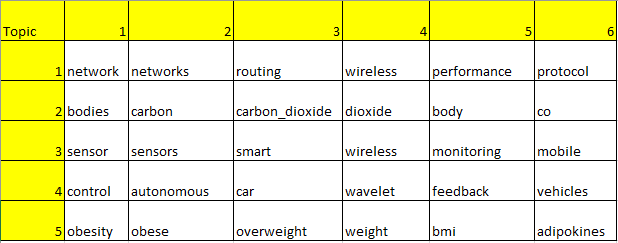
\includegraphics[width=0.9\textwidth]{author_topic}
    \caption{5 trong số 200 topics được suy diễn bằng LDA từ dữ liệu CiteSeerX}
    \label{fig:author_topic}
\end{figure}

\noindent
Nhìn vào bảng chủ đề, có thể thấy chủ đề được học lần này tỏ ra khá có ý nghĩa, các từ trong một chủ đề rất gần nhau về mặt ngữ nghĩa. Như vậy, mặc dù chưa cài đặt được mô hình LDA có nhãn, nhưng mô hình này cũng tỏ ra khá hiệu quả. Có triển vọng trong tương lai.


\newpage
\section{Kết luận}
Vậy tất cả những gì đã trình bày cũng là tất cả những gì chúng em đã học được và làm được trong quá trình nghên cứu. Mặc dù tất cả chỉ là kết quả tạm thời, dở dang, nhưng tương lai phát triển cho những gì đã đạt được là hoàn toàn rộng mở. 


Trong tương lai, có thể mô hình Author-Topic sẽ được tìm hiểu chi tiết về cơ sở lý thuyết. Mô hình LLDA sẽ được cài đặt hoàn chỉnh, từ đó vector hóa các bài báo một cách hiệu quả nhất. Tiếp theo sẽ là khai thác dữ liệu mạng, để khai thác dữ liệu này, có thể sử dụng thuật toán PageRank và một số biến thể của nó cho nhiều dạng đồ thị giàu thông tin. Hoặc kết hợp với mô hình nhúng Autoencoder mà nhóm anh Nguyễn Thành Đạt và anh Đinh Xuân Trường đang thực hiện để đưa ra được kết quả tốt nhất.


Cuối cùng, chúng em xin một lần nữa gửi lời cảm ơn chân thành tới cô Nguyễn Kim Anh, cùng mọi người trong nhóm, nhóm anh Nguyễn Thành Đạt và anh Đinh Xuân Trường đã nhiệt tình giúp đỡ, chỉ bảo chúng em trong quá trình thực hiện Project.

\newpage

\begin{thebibliography}{9}
\bibitem{latexcompanion} 
Xiaozhong Liu, Jinsong Zang, Chun Guo
\textit{Citation Recommendation via Proximity Full-Text Citation Analysis and Supervised Topical Prior}. 
Journal of the American Society for Information Science and Technology, 2016.


\bibitem{latexcompanion} 
Walker, D., Xie, H., Yan, K. K., \& Maslov, S. 
\textit{Ranking scientific publications using a model of network
traffic}.  
Journal of Statistical Mechanics: Theory and Experiment, 2007


\bibitem{latexcompanion} 
Dietz, L., Bickel, S., \& Scheffer, T. 
\textit{ Unsupervised prediction of citation influences}.  
Proceedings of the
24th international conference on Machine learning 2007

 
 
\bibitem{latexcompanion} 
J. Dickey.
\textit{ Multiple hypergeometric functions: Probabilistic interpretations and statistical uses}.  
Journal of the American Statistical Association, 1983.



\bibitem{latexcompanion} 
M. Abramowitz and I. Stegun, editors.
\textit{ Handbook of Mathematical Functions}.  
Dover, New York, 1970.


\bibitem{latexcompanion} 
Daniel Ramage, David Hall, Ramesh Nallapati and Christopher D. Manning.
\textit{ Handbook of Mathematical Functions}.  
Computer Science Department
Stanford University 2009


\bibitem{latexcompanion} 
Michal Rosen-Zvi
\textit{The Author-Topic Model for Authors and Documents}.  
Computer Science Department
Stanford University 2004

\end{thebibliography}



\end{document}